%!TEX root = ../template.tex
%%%%%%%%%%%%%%%%%%%%%%%%%%%%%%%%%%%%%%%%%%%%%%%%%%%%%%%%%%%%%%%%%%%%
%% chapter4.tex
%% NOVA thesis document file
%%
%% Chapter with lots of dummy text
%%%%%%%%%%%%%%%%%%%%%%%%%%%%%%%%%%%%%%%%%%%%%%%%%%%%%%%%%%%%%%%%%%%%

\typeout{NT FILE chapter4.tex}%

\chapter{Proposal}
\label{cha:proposal}

\section{Adaptation protocol} % (fold)
\label{sec:adaptation_protocol}

\section{Service Registry} % (fold)
\label{sec:service_registry}

The service contracts are written in standard specification language such as OpenAPI;

Each operation's signature in every contract can be expressed as a function.
For each pair of versions (new, old) a compatibility specification file is produced;

In this file all functions and parameters are associated with a key;

Records are expanded/exploded and each of its parameters is associated with a key, the record itself is also associated with a key;

This file contains the associations between the old version function/parameter keys, and the new version parameters keys (eg. old:k0 -> new:k1; old:k1->new:k5);

This file is audited by a programmer before being used for the generation of the adapter proxy code
In case of incorrect mapping between parameter types the programmer can fix manually.

Some ambiguous evolutions can only be solved with human intervention and knowledge of the domain;
The system notifies the programmer if such a case occurs and request intervention for its resolution.

Examples:
renaming two fields of the same type;
inserting a new field and removing another of the same type, is indistinguishable from renaming a field;

Default values can also be supplied inside compatibility specification in order to de-clutter service API or implementations;

More complex signature changes (such as the change of parameter unit from celsius to fahrenheit, the change of date format, the partition of name parameter into surname and first name)
can be accommodated in the combinability specification with the use of functions (eg. extractFirstName(old:k0) -> new:k1  extractSurname(old:k0) -> new:k1)

This functions can be made available through static libraries, or more interestingly, the programmer could write their implementation in the compatibility specification file
and afterwards they would be integrated in adapter proxy coded before compilation;

The versions of service API are collected in a schema registry;

When a new version is submitted for deployment the registry is consulted in order to obtain the set of all active versions of the same service;

\begin{figure}[htbp]
    \centering
    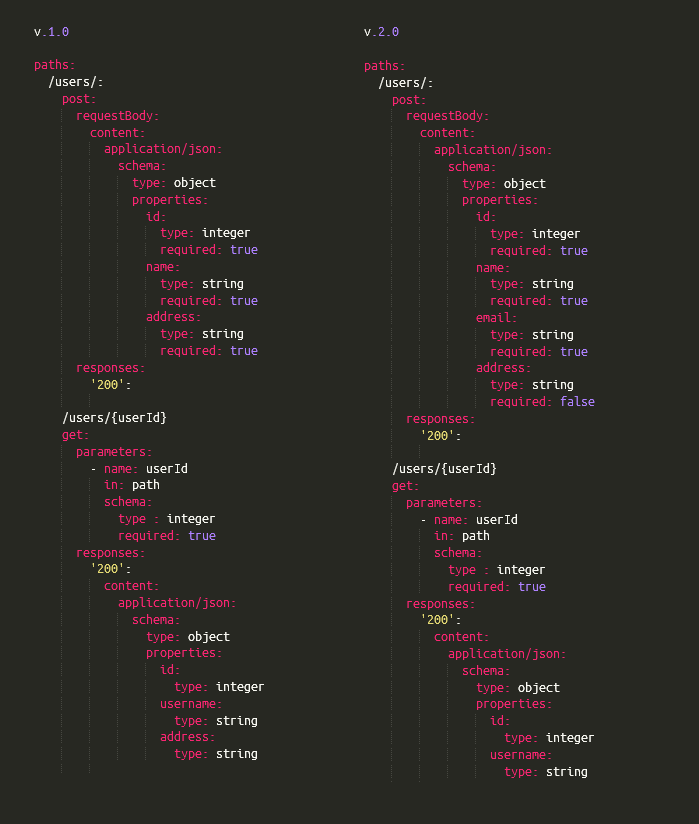
\includegraphics[height=5.7in]{simple_sig}
    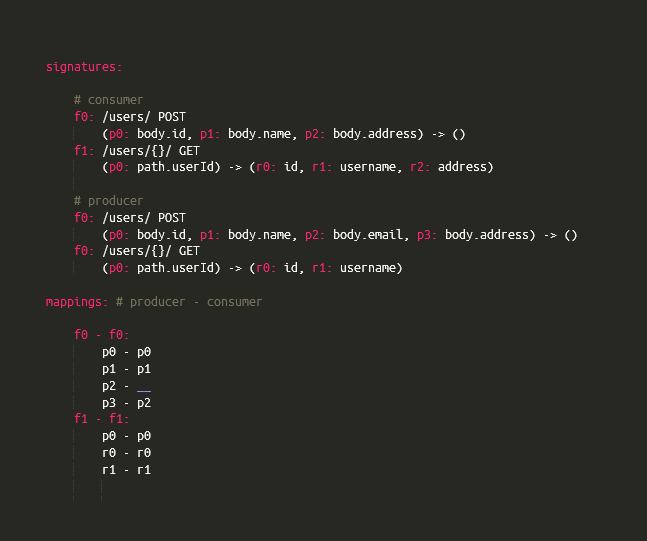
\includegraphics[height=4in]{map}
    \caption{Service contracts}
    \label{fig:simple}
\end{figure}

\section{Benchmark platform} % (fold)
\label{sec:benchmark_platform}

The platform's main requirement is the ability to evaluate different solutions in comparable scenarios while utilizing the same evaluation criteria. It must also be capable of evaluating a solution without requiring modifications to an existing implementation.

Experiments must be simple to share and reproduce by different individuals.

It should be straightforward to aggregate reported metrics for a certain time period between two events, such as the beginning and conclusion of the evolution of a service.

The platform must allow users to specify how and when each service should evolve via a pipeline configuration file or directly through a terminal.

\paragraph{Approaches under assessment}

\paragraph{Rollover deployments}
A rolling deployment is a deployment strategy that slowly replaces previous versions of an application with new versions.
A new batch of instances is launched before taking the old instances out of service.

\paragraph{Data-serialization languages with schema evolution support }
Frameworks such as Protobuf, Thrift, and Avro offer data schema evolution, although their support is severely limited and lacks assurances about the safety of deployment operations.

\paragraph{Proxy Adapter}
A proxy is injected into a micro-service image, which intersects all requests and responses and modifies messages, allowing involved services to communicate without subscribing to the same contract version.

\paragraph{Benchmark platform architecture}

\begin{figure}[htbp]
    \centering
    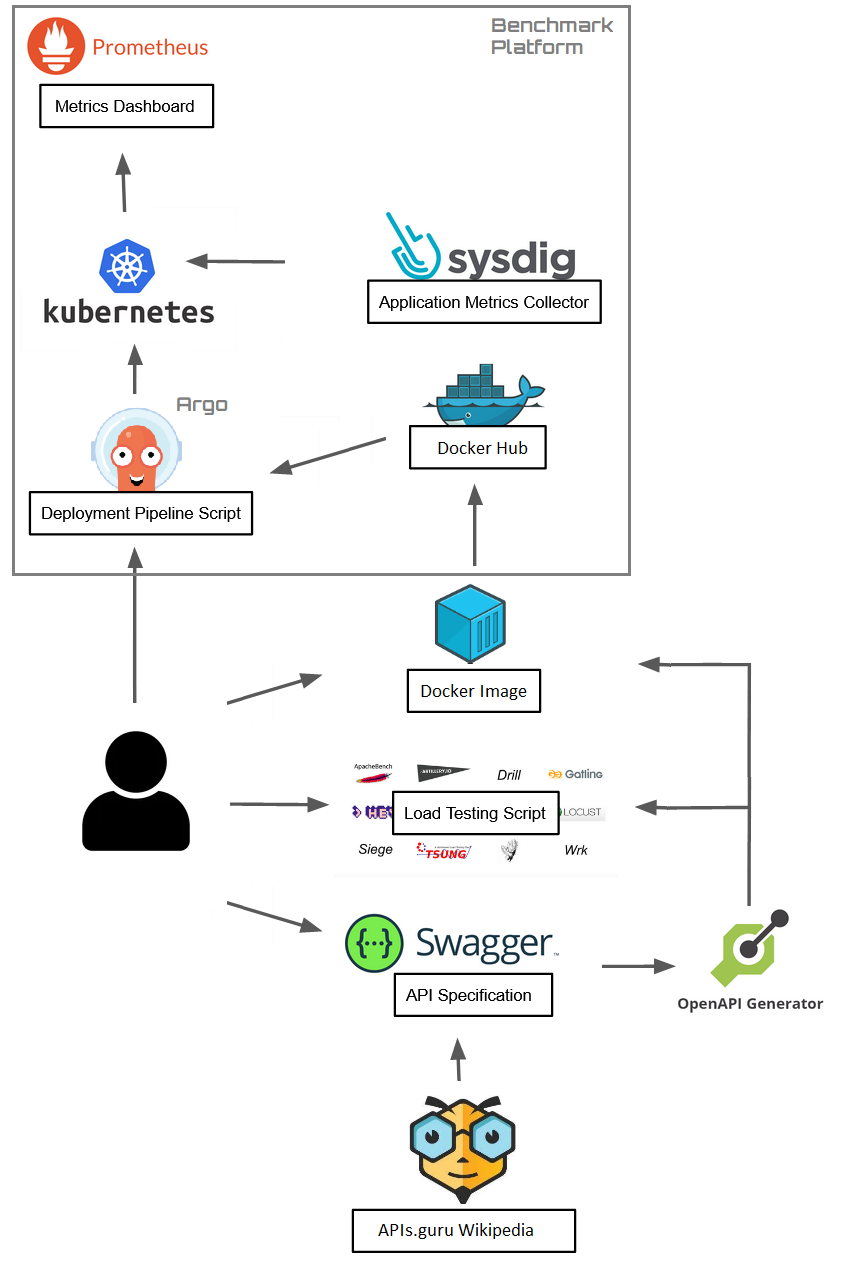
\includegraphics[height=3in]{canvas}
    \caption{The figure illustrates the benchmark platform components}
    \label{fig:canvas}
\end{figure}

\paragraph{Services evolution} can be specified in a Argo workflow through tasks.
Argo is a robust pipeline engine for Kubernetes, It provides simple, flexible mechanisms for specifying constraints between tasks and for linking the output of any task as an input to subsequent task.

Complex experiments can be made with Argo since the state of each deployment in Kubernetes can be queried via a task and utilized as input in a decision that leads to different tasks.

\paragraph{Active virtual users} The Argo workflow file may be used to specify how and when each service should evolve, as well as to manage active virtual users by deploying and stopping docker images that contain load testing scripts.


\paragraph{Test Implementations}
Developing implementations (for a specific evolution strategy) is a time-consuming endeavor because several versions of the same app are required to test its evolution.
API.guro contains the APIs for a few apps in various versions.
The open-AI generator project can produce bare-bones server implementations based on the swagger specification of a app.
The produced implementation does nothing by default; modifications would be required for services to be able to discover and communicate with one another.
It will be necessary to choose application APIs and develop each application service in several versions.

\paragraph{Results}
Metrics are collected via the kubernetes logging API that is accessed by Promotheus. Prometheus is a pull-based monitoring system. It periodically sends HTTP scrape requests, the response to this requests is parsed in storage along with the metrics for the scrape itself.
Kurbenetes does not gather application-specific metrics by default, such as latency and error rate. Sysdig monitor fixes this problem without needing application instrumentation by leveraging the eBPF protocol to obtain information about all system calls straight from the kernel.
With the conjunction of this tools is possible to evaluate the latency, error rate, traffic, and saturation of each service individually in an event-based time series.

Gathered data may be visualized in real-time using Grafana dashboards, that can be customized through Prometheus.
Prometheus provides a query language that allows metrics to be aggregated by events or components.
Raw data from Prometheus can also be downloaded.